\begin{filecontents*}{example.eps}
%!PS-Adobe-3.0 EPSF-3.0
%%BoundingBox: 19 19 221 221
%%CreationDate: Mon Sep 29 1997
%%Creator: programmed by hand (JK)
%%EndComments
gsave
newpath
  20 20 moveto
  20 220 lineto
  220 220 lineto
  220 20 lineto
closepath
2 setlinewidth
gsave
  .4 setgray fill
grestore
stroke
grestore
\end{filecontents*}
%
\documentclass[smallextended,natbib,runningheads]{svjour3}
%
\journalname{Computational Statistics}
%
\smartqed  % flush right qed marks, e.g. at end of proof
%
\usepackage{amsmath}
\usepackage{amssymb}
\usepackage{graphicx}
\usepackage{epstopdf}% To incorporate .eps illustrations using PDFLaTeX, etc.
\usepackage{subfigure}% Support for small, `sub' figures and tables
\usepackage{multirow}
\usepackage{float}
\usepackage{xcolor}
\usepackage{comment}
\usepackage{natbib}% Citation support using natbib.sty
\newcommand{\f}{\operatorname}
\newcommand{\R}{\mathbb{R}}
\newcommand{\N}{\mathbb{N}}
\newcommand{\bs}{\boldsymbol}

% \usepackage{mathptmx}      % use Times fonts if available on your TeX system
%
% insert here the call for the packages your document requires
%\usepackage{latexsym}
% etc.
%
% please place your own definitions here and don't use \def but
% \newcommand{}{}
%
\begin{document}

\title{Reference posterior properties with censored response using the Gamma distribution
}


%\titlerunning{Short form of title}        % if too long for running head

\author{Eduardo Ramos         \and
        Pedro Luiz Ramos \and Jeremais Leão \and Francisco Louzada%etc.
}

%\authorrunning{Short form of author list} % if too long for running head

\institute{E. Ramos \at
              Departamento de Estat\'istica, Universidade Federal do Amazonas, Manaus, Brazil \\           %  \\
%             \emph{Present address:} of F. Author  %  if needed
           \and
           P.L. Ramos \at
              Facultad de Matem\'aticas, Pontificia Universidad Cat\'olicade Chile, Santiago, Chile
 \email{pedro.ramos@mat.uc.cl}
 \and 
 J.Leão \at 
Departamento de Estat\'istica, Universidade Federal do Amazonas, Manaus, Brazil \\
 \and 
 F. Louzada \at 
 Institute of Mathematical Science and Computing, University of S\~ao Paulo, S\~ao Carlos, Brazil \\
}




\date{Received: date / Revised: date}
% The correct dates will be entered by the editor


\maketitle

\begin{abstract}
This research investigates the properties of the posterior distribution of the Gamma distribution, especially in the context of censored data. We establish necessary and sufficient conditions for determining when improper priors lead to proper posteriors. Additionally, we derive conditions to ascertain the finiteness of the posterior moments. The study addresses the challenges posed by censoring and delves into the application of various objective priors. We introduce a novel estimator for censored data, enhancing the efficiency of the Markov Chain Monte Carlo (MCMC) algorithm. Through a simulation study, we evaluate the performance of Bayesian estimators under different priors. Our methodology is applied to a dataset from the Cancer Genome Atlas, focusing on lung adenocarcinoma in patients over 70, offering valuable insights into disease progression and mortality patterns.
\keywords{censored data \and gamma distribution\and objective priors \and closed-form estimators.}
\end{abstract}

\section{Introduction}



The gamma distribution is a significant generalization of the exponential model and is widely employed in reliability and survival studies. Let $T$ be a non-negative random variable with a gamma distribution. Its probability density function is given by
\begin{equation*}%\label{fdpgamma}
f(t|\phi,\mu)= \frac{\mu^\phi}{\Gamma(\phi)}t^{\phi-1}\exp(-\mu t) ,\quad t>0
\end{equation*}
where $\phi>0$ and $\mu>0$ are the unknown shape and scale parameters, respectively, and $\Gamma(\phi)=\int_{0}^{\infty}{e^{-u}u^{\phi-1}du}$ is the complete gamma function. 

Numerous frequentist methods have been proposed for parameter estimation of the gamma distribution, with the maximum likelihood method being the primary choice in practical applications. \cite{ye2017closed} proposed closed-form estimators based on maximum likelihood, which are straightforward to compute.  \cite{wang2018inference} developed inferential procedures, including a confidence interval for the shape parameter and generalized confidence intervals to construct prediction limits for a single future measurement. Moreover,  \cite{louzada2019note} introduced bias-free closed-form MLEs and compared them to other methods, demonstrating that their approach provides accurate estimates for complete data, even with small samples.

From the Bayesian perspective, a prior distribution must be chosen for the parameters. Several authors have proposed conjugate and objective priors for the parameters of the gamma distribution considering complete data (see  \cite{son2006bayesian} and the references therein).  \cite{bernardo2005} argued that using simple proper priors, assumed to be noninformative, might obscure crucial and unwarranted assumptions that could dominate or invalidate statistical analysis, thereby recommending against their use.  \cite{northrop2016} emphasized the absence of a universal framework that provides clear criteria for determining when an improper prior leads to a proper posterior distribution in a specific model, highlighting the importance of examining each case individually.  \cite{ramos2021posterior} discussed conditions to determine whether improper priors lead to proper posterior distributions for gamma distributions and applied the results to various objective priors.  \cite{ramos2020power} observed that many objective priors exhibit a power-law behavior, and such a result can be used to determine whether these priors lead to proper posteriors for complete data.


However, when studying time-dependent phenomena, it is common to encounter incomplete or partial information, often referred to as censored data. Despite their partial nature, such data can provide essential information about unknown parameters of interest, and excluding them can result in biased estimates. While there is extensive literature on applying objective priors to complete data, the same approach has not been widely considered in the presence of censoring. \cite{de2001jeffreys} discussed a method to modify the Jeffreys prior to accounting for censored information and applied this approach to the exponential distribution.  \cite{tian2022specifying} provided a comprehensive literature review and demonstrated how to extend and adapt methods for obtaining objective priors suitable for various types of censored data. \cite{ramos2020posterior} discussed conditions for improper priors to yield proper posteriors in the presence of censoring for the Weibull distribution. These results were extendable due to the simple form of the survival function included in the likelihood function.


In this paper, we derive conditions to determine if improper priors lead to proper posteriors and finite higher moments in the presence of multiple censoring times. We modify the likelihood function to account for the partial information, which, for the gamma distribution, involves a product of incomplete gamma functions. This modification complicates the study of the posterior's behavior. Our results generalize the available findings and, as a special case, describe the behavior for complete data. We apply various objective priors to obtain a posterior with properties such as one-to-one invariance, consistent marginalization, and consistent sampling. We obtain posterior summaries using the Markov Chain Monte Carlo (MCMC) methods with the Metropolis-Hastings algorithm. To enhance the convergence of our MCMC, we propose a novel approximate closed-form estimator in the presence of censoring that provides excellent initial values for the iterative method. This estimator simplifies to the standard closed-form MLE, as seen in  \cite{ye2017closed}, in the absence of censoring. To assess the effectiveness of Bayes estimators, we conduct a simulation study comparing their efficiency with maximum likelihood inference for estimating model parameters and examining the potential effect of prior specifications. Finally, to demonstrate our methodology's effectiveness, we apply it to a real-world dataset that describes the lifespan of patients older than 70 years diagnosed with lung adenocarcinoma, aiming to explore the association between this subtype of non-small cell lung cancer and lifespan, offering insights into disease progression and mortality frequency patterns in this specific population.

The remainder of this paper is organized as follows. Section~\ref{sec:2} introduces essential results used to prove the proposed results. We also present a theorem that provides conditions for the posterior distributions to be proper and conditions to determine if the posterior moments of the parameters are finite in the presence of censoring. Section \ref{sec:3} presents the applications of our main theorem to different objective priors. In Section \ref{sec:4}, we discuss an approach to obtain closed-form estimators that initiate the Markov chain Monte Carlo methods, reducing computation time. Section 5 presents the Metropolis-Hastings algorithm to sample from the posterior marginal distributions. A Monte Carlo simulation study in Section 6 compares the effect of different objective priors on the posterior estimates. In Section 7, we apply our approach to a dataset related to the lifespan of patients with lung adenocarcinoma. Finally, Section \ref{sec:6} summarizes the study.

\section{Background}\label{sec:2}

Let $X_1,\ldots,X_n$ be a realization of an independent and identically distributed sample where $X\sim$ Gamma$(\phi,\mu)$. Furthermore, assume that each individual in the sample has both a lifetime $X_i$ and a censoring time $C_i$. Additionally, the censoring times $C_i$ are random and independent of the lifetimes $T_i$, and their distribution is not influenced by the parameters. Under these conditions, the dataset can be described as $(t_i,\delta_i)$, where $T_i=\min(X_i,C_i)$ and $\delta_i=I(T_i\leq C_i)$ is an indicator function of the presence of censoring. The likelihood function in the presence of censoring is given by
\begin{equation*}L(\boldsymbol{\phi,\mu; t,\delta})
=\frac{\mu^{m\phi}}{\Gamma(\phi)^n}\left\{\prod_{i=1}^n{t_i^{\delta_i(\phi-1)}}\right\}\exp\left\{-\mu\sum_{i=1}^n {\delta_i}t_i\right\}\prod_{i=1}^n\left(\Gamma(\phi,\mu t_i)\right)^{1-\delta_i},
\end{equation*}
where $m=\sum_{i=1}^{n}\delta_i$, and $\Gamma(y,x)  =\int_{x}^{\infty}{w^{y-1}e^{-w}dw}$ is the upper incomplete gamma function. Note that $\Gamma(y,0)=\Gamma(y)$, i.e., the incomplete gamma function reduces to the complete gamma function.

Considering a prior distribution $\pi(\phi,\mu)$, the joint posterior distribution for $(\phi,\mu)$ is given by 
\begin{equation}\label{principal}
\pi(\phi,\mu|\boldsymbol{t})=\frac{\pi(\phi,\mu)}{d(\boldsymbol{t,\delta})} \frac{\mu^{m\phi}}{\Gamma(\phi)^n}\left\{\prod_{i=1}^n{t_i^{\delta_i(\phi-1)}}\right\}\exp\left\{-\mu\sum_{i=1}^n {\delta_i}t_i\right\}\prod_{i=1}^n\left(\Gamma(\phi,\mu t_i)\right)^{1-\delta_i},
\end{equation}
where  $d(\boldsymbol{t,\delta})$ is a normalized constant in the form 
\begin{align*}%\label{posteriord2}
d(\boldsymbol{t,\delta})=&\int_{\mathcal{A}} \pi(\phi,\mu)\frac{\mu^{m\phi}}{\Gamma(\phi)^n}\left\{\prod_{i=1}^n{t_i^{\delta_i(\phi-1)}}\right\}\exp\left\{-\mu\sum_{i=1}^n {\delta_i}t_i\right\}\prod_{i=1}^n\left(\Gamma(\phi,\mu t_i)\right)^{1-\delta_i}\; d\boldsymbol{\theta}.
\end{align*}
where $\mathcal{A}=(0,\infty)\times (0,\infty)$ and $\boldsymbol{\theta}=(\phi,\mu)$

%\begin{equation}
%\pi(\phi,\mu|\boldsymbol{t,\delta})=\frac{\pi(\phi,\mu)}{d(\boldsymbol{t,\delta})} \phi^{n\mu}\mu^{n}\left(\prod_{i=1}^n x_i^{\mu}\right)\exp \left\{-\sum_{i=1}^n x_i^\mu \phi^{\mu}\right\},
%\end{equation}
%where $d(\boldsymbol{t,\delta})$ is a normalized constant in the form 
%\begin{equation}\label{posteriord2}
%d(\boldsymbol{t,\delta})=\int_{0}^{\infty}\int_{0}^{\infty}\pi(\phi,\mu)\phi^{n\mu}\mu^{n}\left(\prod_{i=1}^n x_i^{\mu}\right)\exp \left\{-\sum_{i=1}^n x_i^\mu \phi^{\mu}\right\}d\phi d\mu
%\end{equation}

Our goal is to identify the necessary and sufficient conditions that guarantee the posterior distribution is proper for a broad range of priors. To accomplish this, we will use the following propositions as tools. We use $\overline{\mathbb{R}}$ to refer to the extended real number line, which is the union of the real numbers and negative and positive infinity. We use a subscript $*$ to indicate that $0$ is excluded from the sets $\mathbb{R}$ and $\overline{\mathbb{R}}$.

\begin{definition}\label{definition0} Let $\f{g}:I\to\overline{\mathbb{R}}_*^+$ and $\f{h}:I\to\overline{\mathbb{R}}_*^+$, where $I\subset\mathbb{R}$. We say that $\f{g}(x)\propto \f{h}(x)$ if there exists $c_0\in \mathbb{R}^+_*$ and $c_1\in \mathbb{R}^+_*$ such that $c_0\f{h}(x) \leq \f{g}(x) \leq c_1\f{h}(x)$ for every $x\in I$.
\end{definition}

\begin{definition}\label{definition1}
Let $a\in \mathbb{\overline{R}}$, $\f{g}:I\to\mathbb{R^+_*}$ and $\f{h}:I\to\mathbb{R^+_*}$, where $I\subset\mathbb{R}$. We say that $\f{g}(x)\underset{x\to a}{\propto} \f{h}(x)$ if
\begin{equation*}
\liminf_{x\to a} \frac{\f{g}(x)}{\f{h}(x)} > 0\ \mbox{ and }\ \limsup_{x\to a} \frac{\f{g}(x)}{\f{h}(x)} < \infty  \,.
\end{equation*}
The meaning of the relations $\f{g}(x)\underset{x\to a^+}{\propto} \f{h}(x)$ and $\f{g}(x)\underset{x\to a^-}{\propto} \f{h}(x)$ for $a\in \mathbb{R}$ are defined analogously.
\end{definition}

Note that, from the above definition, if for some $c\in \mathbb{R}^+_*$ we have $\lim_{x\to a} \frac{\f{g}(x)}{\f{h}(x)} = c$, then it will follow that $\f{g}(x)\underset{x\to a}{\propto} \f{h}(x)$. The following proposition is a direct consequence of definition \ref{definition1}, where all functions involved are supposed to be positive.

\begin{proposition}\label{properties} For $a\in\overline{\mathbb{R}}$ and $r\in\mathbb{R}$ , let $f_1(x)\underset{x\to a}{\propto} f_2(x)$ and $g_1(x)\underset{x\to a}{\propto} g_2(x)$. Then we have
\begin{equation*}
f_1(x)g_1(x)\underset{x\to a}{\propto}f_2(x)g_2(x) \quad \mbox{ and } \quad f_1(x)^r\underset{x\to a}{\propto}f_2(x)^r.
\end{equation*}

\end{proposition} 

Using the above definitions we can state the following result, which provides necessary as well as sufficient conditions in order for (\ref{principal}) to be proper, and whose proof will be left to the appendix.

\begin{theorem}\label{mainth} Suppose $\pi(\phi,\mu) = \pi(\phi)\pi(\mu)$ for all $\phi>0$ and $\mu>0$, where $\pi(\mu)\propto \mu^k$, $k\in \mathbb{R}$. Then the following is valid:
\begin{itemize}
    \item[(i)] If $k< -1$ then the posterior (\ref{principal}) is improper
    \item[(ii)] If $\lim_{\phi\to 0^+}\pi(\phi)\phi^r = \infty$ for all $r\in \mathbb{N}$, then the posterior (\ref{principal}) is improper
    \item[(iii)] If $k\geq -1$, if $\pi(\phi)$ satisfy
    \begin{equation*} \pi(\phi)\underset{\phi\to 0^+}{\propto} \phi^{r_0}\mbox{ and }\pi(\phi)\underset{\phi\to \infty}{\propto} \phi^{r_\infty},
    \end{equation*}
    and if the uncensored data are not empty nor all equal, then the posterior (\ref{principal}) will be proper as long as $m>-r_0$, in which case all posterior moments for $\phi$ and $\mu$ will be finite.
\end{itemize}

\end{theorem}

\section{Non informative priors}\label{sec:3}



 \cite{jeffreys1946invariant} introduced a method for deriving a non-informative prior that relies on the Fisher information matrix $I(\boldsymbol{\theta})$, where $\boldsymbol{\theta}$ represents the parameter vector. The Jeffreys prior is obtained by taking the square root of the determinant of this matrix. This prior has gained significant popularity due to its appealing property of being invariant under one-to-one transformations of the parameters. In simpler terms, if there exists a one-to-one function $\boldsymbol{\Phi}=\boldsymbol{\Phi}(\boldsymbol{\theta})$, the resulting posterior distribution $p(\boldsymbol{\Phi}|\boldsymbol{t,\delta})$ obtained from the reparametrized model $f(\boldsymbol{t,\delta}|\boldsymbol{\Phi})$ should be consistent with the posterior distribution $p(\boldsymbol{\theta}|\boldsymbol{t,\delta})$ obtained from the original model $f(\boldsymbol{t,\delta}|\boldsymbol{\theta})$, i.e., $p(\boldsymbol{\Phi}|\boldsymbol{t,\delta})=p(\boldsymbol{\theta}|\boldsymbol{t,\delta})|\frac{d\boldsymbol{\theta}}{d\boldsymbol{\Phi}}|$.

The Jeffreys prior can be obtained by taking the square root of the determinant of the Fisher information matrix $I(\boldsymbol{\theta})$ as follows:
\begin{equation}\label{jeffreysp} 
\pi(\boldsymbol{\theta})\propto \sqrt{\det I(\boldsymbol{\theta})}.
\end{equation}
Here, $I(\boldsymbol{\theta})$ represents the $k\times k$ Fisher information matrix, where $I_{ij}(\boldsymbol{\theta})$ is the Fisher information element of $\boldsymbol{\theta}$ in $i$ and $j$  given by
\begin{equation*}%\label{fisherinf1}
I_{ij}(\boldsymbol{\theta})=\f{E}_{\boldsymbol{\theta}}\left[-\frac{\partial^2}{\partial \theta_i \partial \theta_j}\log(L(\boldsymbol{\theta},\boldsymbol{t,\delta}))\right],\ i,j=1,2,\ldots,k.
\end{equation*}

Assuming that the data does not have any censoring the prior has a simple closed-form expression given by
\begin{equation*}%\label{priorjnk}
\pi_J\left(\phi,\mu\right)\propto \frac{\sqrt{\phi\psi'(\phi)-1}}{\mu},
\end{equation*}
where $\psi'(k)=\frac{\partial}{\partial k}\psi(k)$ is the trigamma function.
On the other hand, in the presence of censoring, we need to modify the Fisher information matrix.  \cite{de2001jeffreys} discuss a way to achieve the Fisher information in the presence of different types of censoring, the exact computation of Jeffreys prior under-censored data could be written as
\begin{equation*}
\pi_J^*\left(\phi,\mu\right)=\sqrt{\det(I^*(\boldsymbol{\theta}))},
\end{equation*}
where $\boldsymbol{\theta}=(\phi,\mu)$ and $I^*(\boldsymbol{\theta})$ is given by
\begin{equation*} \{I^*(\boldsymbol{\theta})\}_{h,j} = -[H_D(\theta_h,\theta_j)+H_C(\theta_h,\theta_j)],
\end{equation*}
for $h$ and $j$ assuming the values in $\{1,2\}$, where
\begin{equation*} 
H_D(\theta_h,\theta_j) = \sum_{i=1}^n \f{E}_{\boldsymbol{\theta}}\left[\frac{\partial^2}{\partial \theta_h\partial \theta_j} l_i^D(\boldsymbol{\theta})\right]\f{Pr}\left\{\delta_i=1|\boldsymbol{\theta}\right\}.
\end{equation*}
\begin{equation*}
H_C(\theta_h,\theta_j) = \sum_{i=1}^n \f{E}_{\boldsymbol{\theta}}\left[\frac{\partial^2}{\partial \theta_h\partial \theta_j} L^C_i(\boldsymbol{\theta})\right]\f{Pr}\left\{\delta_i=0|\boldsymbol{\theta}\right\},
\end{equation*}
where $S(y|\boldsymbol{\theta}) = 1-F(y|\boldsymbol{\theta})$, $l_i^D(\boldsymbol{\theta})=\log f(y_i|\boldsymbol{\theta})$, $l_i^C=\log S(y_i|\boldsymbol{\theta})$. Now, we have
\begin{equation*} 
S(t|\boldsymbol{\theta}) = \frac{\Gamma[\phi,(\mu t)]}{\Gamma(\phi)},
\end{equation*}
and thus
\begin{equation*} \f{E}_{\boldsymbol{\theta}}\left[ \frac{\partial^2}{\partial \phi ^2} l_i^C(\boldsymbol{\theta})\right] = \f{E}_{\boldsymbol{\theta}}\left[ \frac{\partial^2}{\partial \phi ^2} \log \Gamma(\phi,\mu t_i)\right]-\psi'(\phi).
\end{equation*}
Thus, from \cite{1990-Geddes} it follows that
    \begin{equation*}
    \begin{aligned}
    \frac{\partial^2}{\partial \phi ^2} \log \Gamma(\phi,\mu t_i) &= \frac{1}{\Gamma(\phi,\mu t_i)^2}\left[\Gamma(\phi,\mu t_i)\frac{\partial^2}{\partial \phi ^2}\Gamma(\phi,\mu t_i) - \left(\frac{\partial}{\partial \phi}\Gamma(\phi,\mu t_i)\right)^2\right]\\
    &=2\mu t_i \frac{T(4,\phi,(\mu t_i))}{\Gamma\left[\phi,(\mu t_i)\right]}-\left(\mu t_i\frac{T(3,\phi,(\mu t_i))}{\Gamma(\phi,\mu t_i)}\right)^2,
    \end{aligned}
\end{equation*}
where $T(m,s,x)$ is a special case of the Meijer G-function:
\begin{equation*} 
T(m,s,x) = G_{m-1,\,m}^{\,m,\,0}\!\left(\left.{\begin{matrix}0,0,\dots ,0\\s-1,-1,\dots ,-1\end{matrix}}\;\right|\,x\right).
\end{equation*}
Thus
\begin{equation*} I_{1,1}^*(\boldsymbol{\theta}) = \int_0^\infty \left(2\mu t \frac{T(4,\phi,(\mu t))}{\Gamma\left[\phi,(\mu t)\right]}-\left(\mu t\frac{T(3,\phi,(\mu t))}{\Gamma[\phi,(\mu t)]}\right)^2\right)\frac{\mu^\phi}{\Gamma(\phi)}t^{\phi-1}\exp(-\mu t)\; dt,
\end{equation*}
which, to the best of our knowledge,  does not have a closed expression. Hence, the problem of finding the explicit formula for the censored Fisher information, as well as the for the censored Jeffreys prior $\pi_J^*\left(\phi,\mu\right)$ is, to the best of our knowledge, intractable. On the other hand, we can prove nonetheless that $\pi_J^*\left(\phi,\mu\right)\leq \pi_J(\phi,\mu)$ for type one of censoring, which, as we will see in the next section, implies in special that $\pi_J^*(\phi,\mu)$ leads to a proper posterior.

\begin{proposition}\label{jeffreycens} For type one of censoring we have $\pi_{J}^*(\phi,\mu)\leq \pi_J(\phi,\mu)$ for all $\phi>0$ and $\mu>0$.
\end{proposition}
\begin{proof} For type one of censoring, the random variable representing the model can be expressed as $(Y_i,\delta_i)$, where $Y_i=\min(T_i,c)$, $\delta_i=\f{I}_{T_i\leq c}$, where $T_1$, $T_2$,$\ldots$ are iid distributions under the two-parameter gamma distribution and $c$ is the constant representing the censoring.

Thus, letting $g:\R^+\to \R^+\times \{0,1\}$ be defined by $g(t)=(g_1(t),g_2(t))$, where
\begin{equation*}
\begin{aligned}
g_1(t) = \min(t,c)\mbox{ and }
g_2(t) = \begin{cases}0,\mbox{ if }x\leq c\\
1\mbox{ otherwise}
\end{cases},
\end{aligned}
\end{equation*}
follows that $(Y_i,\delta_i) = g(T_i)$ for all $i$, but since $g$ is measurable, it also follows that $g$ is a statistic over $T_i$. Thus, denoting as before the Fisher information matrix for uncensored data by $I(\boldsymbol{\theta})$ and the censored data one by $I^*(\boldsymbol{\theta})$ for all $\boldsymbol{\theta}=(\phi,\mu)\in \R^+_*\times \R^+_*$, following \cite{2013-Schervish} (Theorem 2.86, p. 113), the matrix
\begin{equation*} J(\boldsymbol{\theta})=I(\boldsymbol{\theta})-I^*(\boldsymbol{\theta})
\end{equation*}
must be symmetrical positive semi-definite. Additionally, since $I^*(\boldsymbol{\theta})$ is the Fischer information matrix of a distribution, it must also be symmetrical semi-definite. Thus it follows from $I(\boldsymbol{\theta})=I^*(\boldsymbol{\theta})+J(\boldsymbol{\theta})$ and from the Minkowski Determinant Theorem \cite{2010-Marcus} (Theorem 4.1.8, p. 115) that
\begin{equation*} \pi_{J}(\boldsymbol{\theta})=\det(I(\boldsymbol{\theta})) \geq \left(\det\left(I^*(\boldsymbol{\theta})\right)^{1/n} + \det\left(J(\boldsymbol{\theta})\right)^{1/n}\right)^n\geq \det(I^*(\boldsymbol{\theta}))=\pi_{J}^*(\boldsymbol{\theta}) 
\end{equation*}
which proves the result.
\end{proof}

\subsection{A class of objective priors}

Hence due to the limitation in obtaining such priors, we will focus our approach on assuming that the priors are obtained from the uncensored Fisher matrix. Suppose that our aim is to consider a fully objective Bayesian inference for the gamma distribution in the presence of random censoring, one can consider the following class of priors
\begin{equation}\label{postunnk1} 
\pi_C(\phi,\mu|\boldsymbol{t,\delta})\propto\frac{(\phi\psi'(\phi)-1)^{a}}{\mu^{b}\phi^{c}}.
\end{equation}

It is worth mentioning that the prior mentioned above is considered a general family of priors used to prove the properties of the posterior distribution. The objective priors obtained from formal rules, such as Jeffreys' prior and reference priors, which depend on the model, will be derived further. As we will see, they are particular cases of the family mentioned above.
The joint posterior distribution for $\phi$ and $\mu$, produced by the class of priors above is given by:
\begin{align}\label{principal2}
\pi(\phi,\mu|\boldsymbol{t,\delta})\propto& \frac{(\phi\psi'(\phi)-1)^{a}\mu^{m\phi-b}}{\phi^{c}\Gamma(\phi)^n}\left\{\prod_{i=1}^n{t_i^{\delta_i(\phi-1)}}\right\}\exp\left\{-\mu\sum_{i=1}^n {\delta_i}t_i\right\}\nonumber\\ 
&\times\prod_{i=1}^n\left(\Gamma(\phi,\mu t_i)\right)^{1-\delta_i},
\end{align}

\begin{theorem}\label{principalnow} The posterior density (\ref{principal2}) is improper in case $b>1$ and will be proper if $b\leq 1$ and $m>a+c$ in case the uncensored data are not empty nor all equal, in which case the posterior moments for $\phi$ and $\mu$ are finite.
\end{theorem}
\begin{proof} From item $(i)$ of Theorem \ref{mainth}, if $b>1$ then the posterior density (\ref{principal2}) is improper. Now, following \cite{Pedro2020onposterior} it follows that
\begin{align*}
\phi \psi'(\phi) - 1 \underset{\phi\to 0^+}{\propto} \phi^{-1}\mbox{ and }
\phi\psi'(\phi) - 1 \underset{\phi\to \infty}{\propto} \phi^{-1}.
\end{align*}
Thus, $\pi_C(\phi,\mu|\boldsymbol{t,\delta})\propto \pi(\phi)\pi(\mu)$ where $\pi(\mu)\propto \mu^{-b}$ and where, due to Proposition \ref{properties}, $\pi(\phi)$ satisfy the conditions of item $(iii)$ of Theorem \ref{mainth} for $r_0=r_\infty=-(a+c)$. Thus, under the second set of hypothesis, since $m>-r_0=a+c$, the posterior (\ref{principal2}) will be proper and the posterior moments for $\phi$ and $\mu$ will be finite.
\end{proof}

One can obtain a basic non-informative prior by using uniform priors that range from $(0,\infty)$. In this case, assuming both $a=b=c=0$, our prior reduces to $\pi_1(\phi,\mu|\boldsymbol{t,\delta})\propto 1$. However, such prior may not be  desirable due to its lack of invariance to reparametrizations.

Note $\pi_J\left(\phi,\mu\right) \propto \pi_C(\phi,\mu|\boldsymbol{t,\delta})$ for $a=\frac{1}{2}$, $b=1$ and $c=0$, from which we conclude from Theorem \ref{principalnow} that it leads to a proper posterior and finite posterior moments for in case the uncensored times are neither empty nor all equal. From Proposition \ref{jeffreycens} the same conclusions hold for $\pi_J^*\left(\phi,\mu\right)$ for type one censoring.


Jeffreys explored various methods for constructing objective priors, and for $\theta\in(0,\infty)$ he proposed the prior $\pi(\theta)=\theta^{-1}$ (see  \cite{kass1996selection}). The main argument behind this choice was the prior's invariance under power transformations of the parameters. As the parameters of the Gamma distribution lie within the interval $(0,\infty)$, the Jeffreys prior can be obtained by setting $a=0$, $b=c=1$.  \cite{miller1980bayesian}, on the other hand, examined another objective prior for the gamma distribution parameters, but choose a prior that leads to a posterior that requires fewer computational subroutines. This alternative prior can be obtained by setting $a=c=0$, $b=1$.

The priors cited above lack the invariance property under one-to-one transformations as discussed at the beginning of this section. An alternative prior was proposed by  \cite{bernardo1979a}  to derive a new class of objective priors, known as reference priors. Subsequently, several studies have been conducted to provide rigorous definitions and derive a class of prior distributions in various contexts (see \cite{berger2015} and the references therein). The reference prior is obtained by maximizing the Kullback-Leibler (KL) divergence, subject to certain regularity conditions. By doing so, the prior is expected to provide the maximum influence to the data on the posterior distributions. The reference priors have important properties such as consistency under sampling, marginalization, and one-to-one transformation invariance, see \cite{bernardo2005}. 

\begin{proposition}\label{propositionop} [ \cite{bernardo2005}, pg 40, Theorem 14]. Let $\boldsymbol\theta=(\theta_1,\theta_2)$ be a vector of the ordered parameters of interest and $I(\theta_1,\theta_2)$ is the Fisher information matrix. If the parameter space  of $\theta_1$ does not depend of $\theta_2$ and $I_{j,j}(\boldsymbol\theta), j=1,2$ are factorized in the form 
\begin{equation*}
S_{1,1}^{-\frac{1}{2}}(\boldsymbol\theta)=f_1(\theta_1)g_1(\theta_2) \ \ \mbox{ and } \ I_{2,2}^{\frac{1}{2}}(\boldsymbol\theta)=f_2(\theta_1)g_2(\theta_2) . 
\end{equation*}
Then the reference prior for the ordered parameters $\boldsymbol\theta$ is given by $\pi_{\boldsymbol\theta}(\boldsymbol\theta)=f_1(\theta_1)g_2(\theta_2)$ and there is no need for compact approximations, even if the conditional priors are not proper.
\end{proposition} 

For example, in the case of the gamma distribution, the overall reference prior is obtained as:
\begin{equation*}%\label{prioroverallf}
\pi_R\left(\phi,\mu\right)\propto \frac{1}{\mu}\sqrt{\frac{\phi\psi'(\phi)-1}{\phi}}.
\end{equation*}

\cite{tibshirani1989noninformative} introduced an alternative method to derive a class of objective priors denoted by $\pi\left(\theta_1, \theta_2\right)$, where $\theta_1$ is the parameter of interest. These priors ensure that the credible interval for $\theta_1$ has a coverage error of $\mathcal{O}\left(n^{-1}\right)$ in the frequentist sense, as expressed by the following equation:
\begin{equation}\label{matchingp}
P\left[\theta_1\leq\theta_1^{1-\xi}\left(\pi;\boldsymbol{x}\right) \mid \left(\theta_1,\theta_2\right)\right] =
1-\xi-\mathcal{O}\left(n^{-1}\right),
\end{equation}
where $\theta_1^{1-\xi}\left(\pi;\boldsymbol{x}\right) \mid \left(\theta_1,\theta_2\right)$ represents the $(1-\xi)$-th quantile of the posterior distribution of $\theta_1$. Priors that satisfy the equation (\ref{matchingp}) are referred to as matching priors.  \cite{tibshirani1989noninformative} demonstrated that the matching priors can be obtained if $\theta_1$ and $\theta_2$ are orthogonal parameters according to the definition given by \cite{cox1987parameter}, i.e., $I_{\theta_1, \theta_2}\left(\theta_1, \theta_2\right)=0$, where $\theta_1$ is the parameter of interest and $\theta_2$ is the orthogonal nuisance parameter. All matching priors can be expressed as priors of the form.
\begin{equation*}%\label{priorgmtb1f}
\pi_{T}\left(\phi,\mu\right)\propto \frac{\phi\psi'(\phi)-1}{\mu\sqrt{\phi}}.
\end{equation*}
which is the prior given in (\ref{postunnk1}) with $c=0.5$, $a=b=1$ and therefore, returns a proper posterior and finite posterior moments under the usual condition on the uncensored times being not empty nor all equal.


There are other ways to achieve objective priors. For instance,  \cite{zellner1,zellner2} proposed an objective prior that is characterized by relatively low information compared to the available data. This prior, called the Maximal Data Information (MDI) prior, can be derived by solving the negative of the Shannon entropy and taking its exponential. For the gamma distribution (see  \cite{ramos2020posterior} for a detailed discussion), this prior is given by:
\begin{equation*}%\label{priorznk2}
\pi_Z(\phi, \mu)\propto\frac{\mu}{\Gamma(\phi)}\exp\left\{(\phi-1)\psi(\phi)-\phi\right\}.
\end{equation*}

As a direct application of Theorem \ref{mainth} we have:
%{\color{red}
\begin{theorem} The prior $\pi_z(\phi,\mu)$ leads to an improper posterior for all $n\geq 1$.
\end{theorem}
\begin{proof} Indeed,  letting $\pi_Z(\phi) = \frac{\exp\left\{(\phi-1)\psi(\phi)-\phi\right\}}{\Gamma(\phi)}$, from \cite{ramos2021posterior} it follows that 
\begin{equation*} \lim_{\phi\to 0^+}\pi_Z(\phi)\phi^r = \infty\mbox{ for all }r\in \mathbb{N}.
\end{equation*}
Thus, from item $(ii)$ of Theorem \ref{mainth} the result follows.
\end{proof}
%}
Therefore, the obtained posterior in the censored case is also improper and should not be used.



\section{Closed-form initial value}

The choice of initial values is an important task when using iterative methods. In order to obtain good initial values we can use a modification of the maximum likelihood method. \cite{ramos2021modified} proposed a generalized closed-form maximum likelihood approach to derive closed-form expressions. Their method relies on identifying a generalized version that can construct such estimators. In this context, we consider a generalized version of the gamma distribution given by
\begin{equation*} f(t| \bs{\theta}) = \frac{\alpha}{\Gamma(\phi)} \mu^{\alpha \phi}t^{\alpha\phi-1}\exp\left[-(\mu t)^\alpha\right],
\end{equation*}
where $\bs{\theta}=(\alpha,\mu,\theta)$, and the likelihood function in the presence of censoring is given by
\begin{equation*}L(\boldsymbol{\theta; t,\delta})
=\frac{\alpha^m\mu^{m\alpha\phi}}{\Gamma(\phi)^n}\left\{\prod_{i=1}^n{t_i^{\delta_i(\alpha\phi-1)}}\right\}\exp\left\{-\mu^{\alpha}\sum_{i=1}^n {\delta_i}t_i^{\alpha}\right\}\prod_{i=1}^n\left(\Gamma[\phi,(\mu t_i)^{\alpha}]\right)^{1-\delta_i},
\end{equation*}
where $m=\sum_{i=1}^{n}\delta_i$.  \cite{louzada2018efficient}, used the idea above jointly with an objective prior to achieving closed-form maximum a posterior estimates that are nearly unbiased. However, in our case and assuming censored data, computing the likelihood equations from the expression above will not return closed-form expressions the partial derivatives from the incomplete gamma function has a complex structure. On the other hand, the incomplete gamma function can be approximated (see  \cite{abramowitz}) by
\begin{equation*} \Gamma(s,x) = x^{s-1}e^{-x}\sum_{k=0}^{\infty} \frac{\Gamma(s)x^{-k}}{\Gamma(s-k)},
\end{equation*}
as our aim is to find a useful initial value we can consider a preliminary approximation, we assume the first-order approximation, that is
\begin{equation*}\Gamma(\phi,(\mu t_i)^\alpha) \approx (\mu t_i)^{\alpha(\phi-1)}e^{-(\mu t_i)^{\alpha}}.
\end{equation*}
Using this approximation, the likelihood function is reduced to
\begin{equation*}L(\bs{\theta;t,\delta})
=\frac{\alpha^m\mu^{n\alpha(\phi-1)+m\alpha}}{\Gamma(\phi)^n}\left\{\prod_{i=1}^n{t_i^{\delta_i(\alpha\phi-1)+(1-\delta_i)\alpha(\phi-1)}}\right\}\exp\left\{-\mu^{\alpha}\sum_{i=1}^n t_i^{\alpha}\right\}.
\end{equation*}
Therefore, assuming the joint prior distribution for $\alpha$, $\mu$ and $\phi$ given by $\frac{1}{\alpha\mu\phi}$, the joint posterior for $\alpha$, $\mu$ and $\phi$ is given by
%{\color{red}
\begin{align*}%\label{postclosedform}
\pi(\alpha,\mu,\phi|\bs{t;\delta})
=&\frac{c\alpha^{m-1}\mu^{n\alpha(\phi-1)+m\alpha-1}}{\phi\Gamma(\phi)^n}\left\{\prod_{i=1}^n{t_i^{\delta_i(\alpha\phi-1)+(1-\delta_i)\alpha(\phi-1)}}\right\}\nonumber \\
&\times \exp\left\{-\mu^{\alpha}\sum_{i=1}^n t_i^{\alpha}\right\},
\end{align*} %}
where $c$ is a normalizing constant. Thus, the joint posterior for $\alpha$ and $\phi$ is given by
%{\color{red}
\begin{align*}\pi(\alpha,\phi|\bs{t,\delta})
=&\frac{c\alpha^{m-1}}{\phi\Gamma(\phi)^n}\left\{\prod_{i=1}^n{t_i^{\delta_i(\alpha\phi-1)+(1-\delta_i)\alpha(\phi-1)}}\right\}\nonumber\\
&\times \int_{0}^\infty \mu^{n\alpha(\phi-1)+m\alpha-1} \exp\left\{-\mu^{\alpha}\sum_{i=1}^n t_i^{\alpha}\right\}d\mu,
\end{align*}
%}
which, using the transformation $v=\mu^{\alpha}$, leads us to
\begin{equation*}%\label{proveproper}
\pi(\alpha,\phi|\bs{t,\delta})
=\frac{c\alpha^{m-2}\Gamma\left[n(\phi-1)+m\right]}{\phi\Gamma(\phi)^n(\sum_{i=1}^n t_i^\alpha)^{n(\phi-1)+m}} \left\{\prod_{i=1}^n{t_i^{\delta_i(\alpha\phi-1)+(1-\delta_i)\alpha(\phi-1)}}\right\}.
\end{equation*}

Thus the closed-form expression from $\phi$ can be obtained from ${\partial \log \pi(\alpha,\phi|\bs{t,\delta})}{/ \partial \alpha}$, that is given by
\begin{equation*}
\begin{aligned} \frac{\partial \log \pi(\alpha,\phi|\bs{t,\delta})}{\partial \alpha} = \frac{m-2}{\alpha} - \frac{(n(\phi-1)+m)\sum_{i=1}^n t_i^{\alpha}\log t_i}{\sum_{i=1}^n t_i^\alpha} + \sum_{i=1}^n (\phi+\delta_i-1) \log t_i.
\end{aligned}
\end{equation*}
By letting $\alpha=1$ we recapture the gamma distribution and letting $\dfrac{\partial\log \pi(\alpha,\phi|\bs{t,\delta})}{\partial \alpha}=0$, after some algebraic manipulation we obtain
\begin{equation}\label{init1} 
\tilde{\phi} = \frac{(m-2) - \sum_{i=1}^n(1-\delta_i)\log t_i + (n-m)\Lambda(\bs{x}) }{n\Lambda(\bs{x})-\sum_{i=1}^n \log t_i}, 
\end{equation}
where $\Lambda(\bs{x}) = \left(\sum_{i=1}^n t_i\log t_i\right)\left(\sum_{i=1}^n t_i\right)^{-1}$. To obtain a closed-form estimator for $\mu$ we need to solve 
\begin{equation*}
\begin{aligned}
\frac{\partial \log \pi(\alpha,\phi|\bs{t,\delta})}{\partial \mu} = \frac{ n(\phi-1)+m}{\mu} -  \sum_{i=1}^n t_i,
\end{aligned}
\end{equation*}
and setting $\partial \log L(\bs{\theta};\bs{t,\delta}) /\partial \mu=0$, and after some algebraic manipulations we have
\begin{equation}\label{init2}
\tilde{\mu} = \frac{n(\tilde{\phi}-1)+m}{\sum_{i=1}^n t_i}
\end{equation}
which has a closed-form expression. Therefore, we compute sequentially $\tilde{\phi}$ and $\tilde{\mu}$. The estimators take into account the censored information, however, as we only considered the first-order approximation of the incomplete gamma function the obtained results may have a small bias.


\section{Sampling from the posterior}

In this section, we outline the Monte Carlo Markov chain algorithm for sampling from the joint posterior distribution.  To generate samples of $\phi$ and $\mu$ from the marginal posterior distribution, the Metropolis-Hastings (MH) algorithm is required since the marginal distributions do not have closed-form expressions. Therefore, in order to obtain samples from the marginal distributions, we can use the conditional distribution given by 
\begin{equation}\label{cond1}
\pi(\phi|\mu,\boldsymbol{t,\delta})\propto \frac{(\phi\psi'(\phi)-1)^{a}}{\phi^{c}\Gamma(\phi)^n}\left\{\prod_{i=1}^n{t_i^{\delta_i(\phi-1)}}\left(\Gamma(\phi,\mu t_i)\right)^{1-\delta_i}\right\},
\end{equation}
\begin{equation*}%\label{cond2}
\pi(\mu|\phi,\boldsymbol{t,\delta})\propto \mu^{m\phi-b}\prod_{i=1}^n\left(\Gamma(\phi,\mu t_i)\right)^{1-\delta_i}\exp\left\{-\mu\sum_{i=1}^n {\delta_i}t_i\right\}.
\end{equation*}


In this study, we adopt the Gamma distribution $q(\mu^{(j)}|\mu^{(*)},d)$ as a proposal distribution to sample values of the parameters $\mu$ and $\phi$, where $d$ and $k$ are hyperparameters that influence the convergence rate of the algorithm. It's important to note that alternative proposal distributions can be utilized in place of the Gamma model, such as any model that generates values in the positive real line. The subsequent steps detail the execution of the MH algorithm:

\begin{enumerate}
\item Compute the initial values of $\phi^{(1)}$ and $\mu^{(1)}$ from (\ref{init1}) and (\ref{init2}) and initialize a counter $j=1$;
\item Generate a random number $\phi^{(*)}$ from the $Gamma(\phi^{(j)}, d)$ distribution;
\item Calculate the acceptance probability, defined as:
\begin{equation*}
\Delta\left(\phi^{(j)},\phi^{(*)}\right)=\min\left(1, \frac{\pi\left(\phi^{(*)}|\mu^{(j)},\boldsymbol{t,\delta}\right)}{\pi\left(\phi^{(j)}|\mu^{(j)},\boldsymbol{t,\delta}\right)} \frac{\f{q}\left(\phi^{(j)},\phi^{(*)}|d\right)}{\f{q}\left(\phi^{(*)},\phi^{(j)}|d\right)}\right),
\end{equation*}
where $\pi(\cdot)$ denotes the conditional posterior distribution of $\phi$ given in (\ref{cond1}). Draw a random sample from an independent uniform distribution $u$ in the interval (0,1);
\item If $\Delta\left(\phi^{(j)},\phi^{(*)}\right)\geq u(0,1)$, accept the value $\phi^{(*)}$ and set $\phi^{(j+1)}=\phi^{(*)}$. If $\Delta\left(\phi^{(j)},\phi^{(*)}\right)< u(0,1)$, reject the value and set $\phi^{(j+1)}=\phi^{(j)}$;

\item Generate a random number $\mu^{(*)}$ from the $Gamma(\mu^{(j)}, k)$ distribution;
\item Calculate the acceptance probability, defined as:
\begin{equation*}
\Delta\left(\mu^{(j)},\mu^{(*)}\right)=\min\left(1, \frac{p\left(\mu^{(*)}|\phi^{(j+1)},\boldsymbol{t,\delta}\right)}{p\left(\mu^{(j)}|\phi^{(j+1)},\boldsymbol{t,\delta}\right)} \frac{\f{q}\left(\mu^{(j)},\mu^{(*)}|k\right)}{\f{q}\left(\mu^{(*)},\mu^{(j)}|k\right)}\right),
\end{equation*}
where $p(\cdot)$ is the conditional posterior $\mu$ distribution given by (\ref{cond1}). Draw a random sample from an independent uniform distribution $u$ in the interval (0,1);
\item If $\Delta\left(\mu^{(j)},\mu^{(*)}\right)\geq u(0,1)$, accept the value $\mu^{(*)}$ and set $\mu^{(j+1)}=\mu^{(*)}$. If $\Delta\left(\mu^{(j)},\mu^{(*)}\right)< u(0,1)$, reject the value and set $\mu^{(j+1)}=\mu^{(j)}$;

\item Increment the counter (j) to (j+1) and repeat steps 2-7 until the chains converge.
\end{enumerate}


From the MH algorithm above we can obtain samples from the marginal posterior distributions of $\mu$ and $\phi$ and compute the posterior summaries. The Bayes estimators are often estimated using one of three metrics: the posterior mean, median, or mode. These estimators are obtained based on distinct loss functions. For example, considering a decision-theoretical perspective, the posterior mean is derived using a mean-square error loss function, while the posterior mode is calculated using a 0-1 loss function. A careful that must be taken is that the while the posterior is proper, its respective mean can be infinite, and therefore it cannot be computed, even using the obtained sample from the MH algorithm. On the other hand, from the main theorem, we have that
\begin{equation*}
\begin{aligned}
E[\phi|\boldsymbol{t,\delta}]=\int_0^{\infty}\int_0^{\infty}&\frac{(\phi\psi'(\phi)-1)^{a}\mu^{m\phi-b}}{\phi^{c-1}\Gamma(\phi)^n}\left\{\prod_{i=1}^n{t_i^{\delta_i(\phi-1)}}\right\}\exp\left\{-\mu\sum_{i=1}^n {\delta_i}t_i\right\}\\&\times\prod_{i=1}^n\left(\Gamma(\phi,\mu t_i)\right)^{1-\delta_i} d\mu d\phi<\infty.
\end{aligned}
\end{equation*}
as well as we have that
\begin{equation*}
\begin{aligned}
E[\mu|\boldsymbol{t,\delta}]=\int_0^{\infty}\int_0^{\infty}&\frac{(\phi\psi'(\phi)-1)^{a}\mu^{m\phi-b+1}}{\phi^{c}\Gamma(\phi)^n}\left\{\prod_{i=1}^n{t_i^{\delta_i(\phi-1)}}\right\}\exp\left\{-\mu\sum_{i=1}^n {\delta_i}t_i\right\}\\&\times\prod_{i=1}^n\left(\Gamma(\phi,\mu t_i)\right)^{1-\delta_i} d\mu d\phi<\infty.
\end{aligned}
\end{equation*}
when $b\geq 1$ and $m>-(a+b)$. Therefore, our approach ensures that the posterior means are proper and can be computed from the MCMC methods.



\section{Numerical evaluation}\label{sec:4}


This section presents a Monte Carlo simulation study to demonstrate the application of our proposed methodology derived in the preceding sections. In order to generate the sample with random censoring, we follow the same steps as described in \cite{ramos2020sampling}. The samples are used to achieve estimates of the parameters via their corresponding Bayesian and classical estimators. Let $\boldsymbol\theta$ represent the parameter vector of size $i=1,2$, and $\hat\theta_{i,1},\hat\theta_{i,2},\ldots,\hat\theta_{i,N}$ denote the respective Bayesian estimates. To evaluate the accuracy of the estimation technique, we adopt the compute the following metrics: mean relative error (MRE), mean squared error (MSE), and coverage probabilities (CP). They are computed, respectively, as
\begin{equation*}%\label{measures}
\text{MRE}_i=\dfrac{1}{N}\sum_{j=1}^{N}\frac{\hat\theta_{i,j}}{\theta_i}, \quad \text{MSE}_i=\dfrac{1}{N}\sum_{j=1}^{N}\left(\hat\theta_{i,j}-\theta_i\right)^2  \ \ \text{and}  \ \ \text{CP}(\theta_i)=\dfrac{\sum_{j=1}^{N} I_{(a,b)}\left(\theta_i\right)}{N}, 
\end{equation*}
where $I_{A}(x)$ means the indicator function, $a=\hat{\theta}_i - z_{\frac{\xi}{2}}\sqrt{H^{-1}_{ii}(\hat{\boldsymbol{\theta}})}$ and $b=\hat{\theta}_i + z_{\frac{\xi}{2}}\sqrt{H^{-1}_{ii}(\hat{\boldsymbol{\theta}})}$, with $z_{\xi/2}$ representing the $\left(\xi/2\right)$-th quantile of a standard normal distribution. 


\begin{table*}[!h]
\centering
\caption{The MRE and (MSE) from the estimates of $\phi=3$ and $\mu=2$ considering different values of $n$, $30\%$ of censoring and with $N=5,000$ simulated samples using the estimation methods: 1 - Initial values (IV), 2 - MLE, 3- Jeffreys Prior, 4 - Reference prior, 5 - Matching prior.}
{\small
\begin{tabular}{c|c|c|c|c|c|c}
\hline
$\boldsymbol{\theta}$ & n & IV & MLE & Jeffreys  & Reference  & Matching  \\
\hline
\multirow{11}{*}{$\phi$} 
&  20 & 0.4886(2.5002) & 1.2256(3.7933) & 1.3604(5.2625) & 1.2322(3.7072) & 1.0953(2.5263) \\
&  30 & 0.5037(2.3060) & 1.1621(2.3775) & 1.2390(2.9566) & 1.1610(2.3364) & 1.0766(1.8218) \\
&  40 & 0.5112(2.2176) & 1.1218(1.5374) & 1.1756(1.8052) & 1.1198(1.5093) & 1.0602(1.2579) \\
&  50 & 0.5144(2.1719) & 1.0995(1.0836) & 1.1437(1.2794) & 1.0984(1.0734) & 1.0514(0.9142) \\
&  60 & 0.5158(2.1524) & 1.0811(0.8661) & 1.1159(0.9783) & 1.0813(0.8567) & 1.0421(0.7568) \\
&  70 & 0.5168(2.1373) & 1.0635(0.6771) & 1.0953(0.7712) & 1.0647(0.6780) & 1.0316(0.6057) \\
&  80 & 0.5184(2.1178) & 1.0584(0.5880) & 1.0869(0.6599) & 1.0590(0.5922) & 1.0315(0.5362) \\
&  90 & 0.5185(2.1139) & 1.0458(0.4917) & 1.0698(0.5410) & 1.0486(0.4963) & 1.0231(0.4526) \\
&  100 & 0.5204(2.0953) & 1.0485(0.4595) & 1.0714(0.5079) & 1.0508(0.4675) & 1.0283(0.4299) \\
&  110 & 0.5209(2.0869) & 1.0414(0.3929) & 1.0621(0.4293) & 1.0437(0.3992) & 1.0235(0.3704) \\
&  120 & 0.5215(2.0806) & 1.0373(0.3443) & 1.0570(0.3794) & 1.0401(0.3504) & 1.0215(0.3258) \\ 
\hline
\multirow{11}{*}{$\mu$} 
&  20 & 0.4962(1.2870) & 1.2953(2.7906) & 1.4778(3.8312) & 1.3197(2.7379) & 1.1534(1.9236) \\
&  30 & 0.5190(1.0908) & 1.2079(1.7215) & 1.3140(2.1381) & 1.2178(1.7067) & 1.1146(1.3414) \\
&  40 & 0.5343(0.9958) & 1.1605(1.1402) & 1.2356(1.3375) & 1.1667(1.1270) & 1.0937(0.9460) \\
&  50 & 0.5393(0.9444) & 1.1306(0.8013) & 1.1919(0.9412) & 1.1363(0.8011) & 1.0789(0.6894) \\
&  60 & 0.5411(0.9232) & 1.1048(0.6268) & 1.1538(0.7117) & 1.1109(0.6251) & 1.0632(0.5551) \\
&  70 & 0.5420(0.9067) & 1.0819(0.4995) & 1.1262(0.5680) & 1.0888(0.5045) & 1.0480(0.4520) \\
&  80 & 0.5431(0.8936) & 1.0719(0.4250) & 1.1117(0.4785) & 1.0775(0.4310) & 1.0436(0.3928) \\
&  90 & 0.5443(0.8823) & 1.0587(0.3613) & 1.0924(0.3979) & 1.0664(0.3670) & 1.0351(0.3366) \\
&  100 & 0.5488(0.8615) & 1.0641(0.3413) & 1.0962(0.3780) & 1.0708(0.3489) & 1.0430(0.3209) \\
&  110 & 0.5478(0.8589) & 1.0514(0.2871) & 1.0804(0.3143) & 1.0577(0.2928) & 1.0331(0.2727) \\ 
&  120 & 0.5511(0.8441) & 1.0510(0.2580) & 1.0784(0.2844) & 1.0577(0.2645) & 1.0346(0.2462) \\
   \hline
\end{tabular}}
\label{tableres1}
\end{table*}


\begin{table*}[!h]
\centering
\caption{The MRE and (MSE) from the estimates of $\phi=3$ and $\mu=2$ considering different values of $n$, $63\%$ of censoring and with $N=5,000$ simulated samples using the estimation methods: Initial values (IV),  MLE, Jeffreys posterior, Reference posterior,  Matching posterior.}
{\small
\begin{tabular}{c|c|c|c|c|c|c}
\hline
$\boldsymbol{\theta}$ & n & IV & MLE & Jeffreys  & Reference  & Matching  \\
\hline
\multirow{11}{*}{$\phi$} 
&  20 & 0.7109(1.2179) & 1.1788(2.3904) & 1.2298(2.7532) & 1.1605(2.2506) & 1.0830(1.7701) \\
&  30 & 0.7146(1.0044) & 1.1164(1.2148) & 1.1494(1.3730) & 1.1045(1.1568) & 1.0565(0.9872) \\
&  40 & 0.7159(0.9219) & 1.0922(0.8251) & 1.1174(0.9175) & 1.0838(0.8040) & 1.0499(0.7097) \\
&  50 & 0.7118(0.8956) & 1.0685(0.5827) & 1.0890(0.6404) & 1.0634(0.5727) & 1.0359(0.5181) \\
&  60 & 0.7096(0.8768) & 1.0475(0.4413) & 1.0643(0.4752) & 1.0448(0.4415) & 1.0216(0.4075) \\
&  70 & 0.7102(0.8515) & 1.0448(0.3626) & 1.0604(0.3936) & 1.0427(0.3631) & 1.0237(0.3397) \\
&  80 & 0.7133(0.8256) & 1.0459(0.3159) & 1.0594(0.3382) & 1.0448(0.3201) & 1.0283(0.2969) \\
&  90 & 0.7104(0.8286) & 1.0369(0.2766) & 1.0500(0.2956) & 1.0361(0.2785) & 1.0214(0.2653) \\
&  100 & 0.7110(0.8190) & 1.0460(0.2583) & 1.0586(0.2821) & 1.0454(0.2604) & 1.0321(0.2464) \\
&  110 & 0.7084(0.8264) & 1.0591(0.2535) & 1.0711(0.2779) & 1.0584(0.2553) & 1.0466(0.2394) \\
&  120 & 0.7087(0.8180) & 1.0779(0.2645) & 1.0893(0.2905) & 1.0780(0.2688) & 1.0663(0.2473) \\
\hline
\multirow{11}{*}{$\mu$} 
&  20 & 0.7716(0.5911) & 1.2126(1.4251) & 1.2817(1.6616) & 1.2066(1.3759) & 1.1218(1.0728) \\
&  30 & 0.7719(0.4281) & 1.1365(0.7130) & 1.1812(0.8142) & 1.1326(0.6895) & 1.0804(0.5895) \\
&  40 & 0.7708(0.3708) & 1.1055(0.4873) & 1.1395(0.5469) & 1.1032(0.4807) & 1.0670(0.4265) \\
&  50 & 0.7688(0.3383) & 1.0831(0.3525) & 1.1106(0.3905) & 1.0829(0.3512) & 1.0534(0.3171) \\
&  60 & 0.7633(0.3222) & 1.0563(0.2625) & 1.0792(0.2845) & 1.0580(0.2654) & 1.0331(0.2445) \\
&  70 & 0.7634 0.3034) & 1.0525(0.2163) & 1.0735(0.2363) & 1.0543(0.2186) & 1.0337(0.2039) \\
&  80 & 0.7671(0.2892) & 1.0530(0.1882) & 1.0709(0.2025) & 1.0553(0.1918) & 1.0377(0.1791) \\
&  90 & 0.7678(0.2772) & 1.0486(0.1662) & 1.0661(0.1794) & 1.0511(0.1685) & 1.0350(0.1598) \\
&  100 & 0.7814(0.2477) & 1.0740(0.1618) & 1.0910(0.1798) & 1.0763(0.1650) & 1.0618(0.1542) \\
&  110 & 0.7957(0.2199) & 1.1092(0.1782) & 1.1255(0.1991) & 1.1112(0.1823) & 1.0981(0.1681) \\
&  120 & 0.8179(0.1841) & 1.1571(0.2281) & 1.1730(0.2549) & 1.1599(0.2343) & 1.1464(0.2145) \\
   \hline
\end{tabular}}
\label{tableres1}
\end{table*}


\begin{table*}[!h]
\centering
\caption{The $CP_{95\%}$ from the estimates of $\phi=3$ and $\mu=2$ considering different values of $n$  with $N=10,000,000$ simulated samples using the estimation methods:  MLE,  Jeffreys Posterior, 4 - Reference posterior, 5 - Matching posterior.}
\begin{tabular}{c|c|c|c|c|c|c|c|c|c}
\hline
\multirow{2}{*}{$\boldsymbol{\theta}$ }  & \multirow{2}{*}{$n$ }  & \multicolumn{2}{c|}{MLE} & \multicolumn{2}{c|}{Jeffreys Prior} & \multicolumn{2}{c|}{Reference Prior}  & \multicolumn{2}{c}{Matching Prior} \\  &  &    $\mu$ & $\theta$ & $\mu$ & $\theta$ & $\mu$ & $\theta$  & $\mu$ & $\theta$ \\
\hline
\multirow{11}{*}{$30\%$} 
&  20 & 0.940 & 0.936 & 0.941 & 0.939 & 0.960 & 0.955 & 0.959 & 0.964 \\
&  30 & 0.941 & 0.938 & 0.932 & 0.933 & 0.947 & 0.946 & 0.947 & 0.949 \\
&  40 & 0.950 & 0.947 & 0.932 & 0.931 & 0.941 & 0.944 & 0.946 & 0.950 \\
&  50 & 0.954 & 0.952 & 0.942 & 0.938 & 0.947 & 0.947 & 0.947 & 0.947 \\
&  60 & 0.957 & 0.955 & 0.944 & 0.941 & 0.950 & 0.950 & 0.949 & 0.950 \\
&  70 & 0.953 & 0.954 & 0.946 & 0.942 & 0.950 & 0.952 & 0.956 & 0.953 \\
&  80 & 0.952 & 0.948 & 0.941 & 0.942 & 0.948 & 0.946 & 0.948 & 0.950 \\
&  90 & 0.951 & 0.947 & 0.943 & 0.943 & 0.947 & 0.946 & 0.947 & 0.948 \\
&  100 & 0.952 & 0.949 & 0.937 & 0.937 & 0.936 & 0.939 & 0.943 & 0.941 \\
&  110 & 0.958 & 0.952 & 0.944 & 0.942 & 0.949 & 0.947 & 0.951 & 0.949 \\
&  120 & 0.954 & 0.956 & 0.946 & 0.943 & 0.949 & 0.949 & 0.948 & 0.948 \\ \hline
\multirow{11}{*}{$60\%$}
&  20 & 0.954 & 0.950 & 0.929 & 0.928 & 0.942 & 0.940 & 0.951 & 0.947 \\
&  30 & 0.959 & 0.957 & 0.938 & 0.939 & 0.948 & 0.945 & 0.949 & 0.951 \\
&  40 & 0.951 & 0.956 & 0.935 & 0.931 & 0.942 & 0.942 & 0.943 & 0.944 \\
&  50 & 0.955 & 0.955 & 0.939 & 0.940 & 0.947 & 0.947 & 0.946 & 0.952 \\
&  60 & 0.954 & 0.952 & 0.946 & 0.947 & 0.946 & 0.951 & 0.949 & 0.951 \\
&  70 & 0.961 & 0.957 & 0.948 & 0.946 & 0.955 & 0.950 & 0.957 & 0.952 \\
&  80 & 0.961 & 0.960 & 0.946 & 0.948 & 0.951 & 0.951 & 0.948 & 0.952 \\
&  90 & 0.953 & 0.961 & 0.945 & 0.950 & 0.949 & 0.950 & 0.947 & 0.952 \\
&  100 & 0.955 & 0.962 & 0.939 & 0.934 & 0.945 & 0.945 & 0.946 & 0.951 \\
&  110 & 0.961 & 0.958 & 0.938 & 0.922 & 0.942 & 0.932 & 0.950 & 0.944 \\
&  120 & 0.954 & 0.937 & 0.927 & 0.881 & 0.930 & 0.893 & 0.939 & 0.906 \\ \hline
\hline
\end{tabular}
\label{tableres2}
\end{table*}

The bias measures the difference between the expected value of the estimator and the true parameter value, while the MSE computes the average of the squared differences between the estimator and the true parameter value. An estimator that yields small values of bias and MSE is generally preferred over one that yields larger values. %Additionally, the coverage probability (CP) is also an important metric. 
For a credibility level of $95\%$ and a large number of experiments, the frequency of intervals that contain the true parameter value should be close to $95\%$. 

The values were generated from a gamma distribution with $\phi=3$ and $\mu=2$, considering $n$ in the range of $20$ to $120$. Additionally, we assumed that the censoring time $C$ follows a uniform distribution, denoted as $C \sim U(0,\lambda)$. For each $x$-th observation generated from a gamma distribution, we have a pair $(T_x, \delta_x)$, where $T_x = \min (X_x, C_x)$ and $\delta_x = \mathrm{I}(X_x \leq C_x)$. Here, $\delta$ is equal to $1$ when the lifetime is observed and $0$ when it is censored (see \cite{ramos2020sampling}). The values of $\lambda$ were set at $5.2$ and $2.2$, which resulted in approximately $30\%$ and $63\%$ censored data, respectively. For each simulated dataset, we conducted 5,500 MCMC iterations. We removed the first 500 samples as a burn-in, with jumps of size 10, to reduce autocorrelation values in the chain. We obtained a chain of 500 samples by discarding these burn-in samples. We evaluated the convergence of the chain using the Geweke criterion [16] with a $95\%$ confidence level. Finally, we computed the posterior medians of $\phi$ and $\mu $ using 10,000 samples.



Based on our findings, we observed that using the approach to obtain closed-form estimators resulted in biased estimates, which was in line with our expectations. Nevertheless, these estimates were highly valuable as they were closer to the true values, enabling the Markov Chain Monte Carlo to operate more efficiently and with a shorter burn-in period. Additionally, it was noted that as the sample size increases, the Mean Relative Error approaches one for all parameter estimators, indicating that they are asymptotically unbiased. Similarly, the Mean Squared Error tends to reach zero for all parameter estimators.

Moreover, the Bayesian approach, utilizing the matching posterior, produced more accurate coverage probabilities through credibility intervals compared to other methods. This was consistent with our expectations based on theoretical results related to coverage probability. Furthermore, in estimating the parameters, the posterior median obtained using the matching posterior provided more precise estimates for the parameters, exceeding the performance of the classical approach.

\section{Application}

In this study, we analyze a sample extracted from the Cancer Genome Atlas (TCGA) dataset. TCGA, a comprehensive dataset derived from a decade-long research project, is accessible through the GDC Data Portal. The original dataset comprises over 11,000 patients diagnosed with 33 different types of cancer. Among these, the most prevalent ones are "breast invasive carcinoma," "kidney clear cell carcinoma," and "lung adenocarcinoma." However, the primary focus of this research is lung adenocarcinoma, a subtype of non-small cell lung cancer. Specifically, the analysis aims to explore the association between lung adenocarcinoma and the lifespan (measured in years) of patients aged over 70 years.

A meticulous investigation of these patients' lifespan is crucial for understanding mortality frequency patterns in this specific population. Analyzing the clinical outcome of lifespan offers valuable insights into disease progression. By examining these data, we can identify significant patterns, relevant trends, and potential prognostic markers, which can be used for risk stratification and personalized medical care. Understanding the relationship between lifespan and lung adenocarcinoma not only aids in clinical decision-making but also contributes to the efficient allocation of healthcare resources, with the goal of enhancing outcomes and the quality of life for patients affected by this particular form of cancer.

To analyze the marginal posterior distributions of $\phi$ and $\mu$, we generated $110,000$ iterations using MCMC methods. The initial values were obtained from equations (\ref{init1}) and (\ref{init2}), yielding $\tilde{\phi}=1.142$ and $\tilde{\mu}=0.214$. We discarded a "burn-in" period of 10,000 values, and set the jumps between consecutive values at a size of 20. As a result, we obtained chains of the marginal posterior distributions, each consisting of 5,000 values. We assessed the convergence of these chains using Geweke's diagnosis \cite{geweke1991evaluating}, which confirmed their convergence. The convergence and autocorrelations were also computed and are available in the supplemental material. Due to the asymmetry of the generated sample, we computed the posterior estimates assuming the posterior median.
\begin{table}[!h]
	\caption{Median, Standard deviation and  $95\%$ credibility intervals for $\mu$, $\phi$ and $y*$}
	\centering % used for centering table
{\small
	{\begin{tabular}{ c | c |  c| c }
			\hline
			$\boldsymbol{\theta}$  & Median & SD & CI$_{95\%}(\boldsymbol{\theta})$ \\ \hline
			\ \ $\mu$ \ \   & 0.2284 &  0.0338  &  (0.1704; 0.3010)  \\ \hline
			\ \ $\phi$   \ \  &  1.2726 & 0.1126 &  (1.0707; 1.5043) \\ \hline
		\end{tabular}}\label{resairplane} }
\end{table}

We consider two commonly used model selection criteria: the BIC (Bayesian or Schwarz Information Criteria) and the AIC (Akaike Information Criteria). The BIC is computed as $\text{BIC} = -2 \ell(\hat{\boldsymbol{\theta}}|\boldsymbol{t,\delta}) + d\log(n)$, while the AIC is given by $\text{AIC} = -2 \ell(\hat{\boldsymbol{\theta}}|\boldsymbol{t,\delta}) + 2d$. In these equations, $d$ represents the number of model parameters, and $\hat{\boldsymbol{\theta}}$ denotes the Bayes estimate of $\boldsymbol{\theta}$. When considering a set of potential models for the available data, the preferred model is the one that yields the lowest values according to these criteria.

\begin{table}[!h]
\centering % used for centering table
	\caption{Results of AIC, and BIC for different probability distributions considering the data set related to the failure time of $194$ of internal cabin mechanical devices in an aircraft.}

	{\begin{tabular}{c|c|c|c|c}
			\hline
			Test   &  Gamma & Weibull & Fréchet & Exponential \\ \hline
			AIC    & \textbf{840.385} & 840.517 & 911.654 & 844.898 \\ 
			BIC    & \textbf{848.234} & 848.366 & 919.503 & 848.822  \\ \hline
		\end{tabular}}\label{discairplane}
\end{table}

The AIC and BIC values for various probability distributions are presented in Table 1. To assess the goodness-of-fit, the empirical survival function (Kaplan-Meier estimate) is compared with the survival functions adjusted by the proposed theoretical models, as illustrated in Figure 1. Upon comparing the adjusted distributions with the empirical survival function, it is evident that the Gamma distribution provides a better fit to the data compared to the competing models. This observation is further supported by the minimum AIC and BIC values obtained for all the analyzed data sets, consistently favoring the Gamma distribution. In order to verify the goodness of fit of the Gamma distribution to the cancer data, we calculate the Cox-Snell residuals \citep{cox1968} defined by
\begin{equation*}
    e_i=-\log \left(\hat S(t_i)\right),\quad  i=1,2,\ldots,n,
\end{equation*}
where $\hat S(t_i)$ is the fitted Gamma survival function of the $i$-th lifetime.  If the Gamma distribution  is correctly specified, then Cox-Snell residuals $e_i$'s are a censored random sample from the standard exponential distribution, that is, $e_i\sim \text{Exp}(1)$, for $i=1,2,\ldots,n$.

\begin{figure*}[!h] 
	\centering
	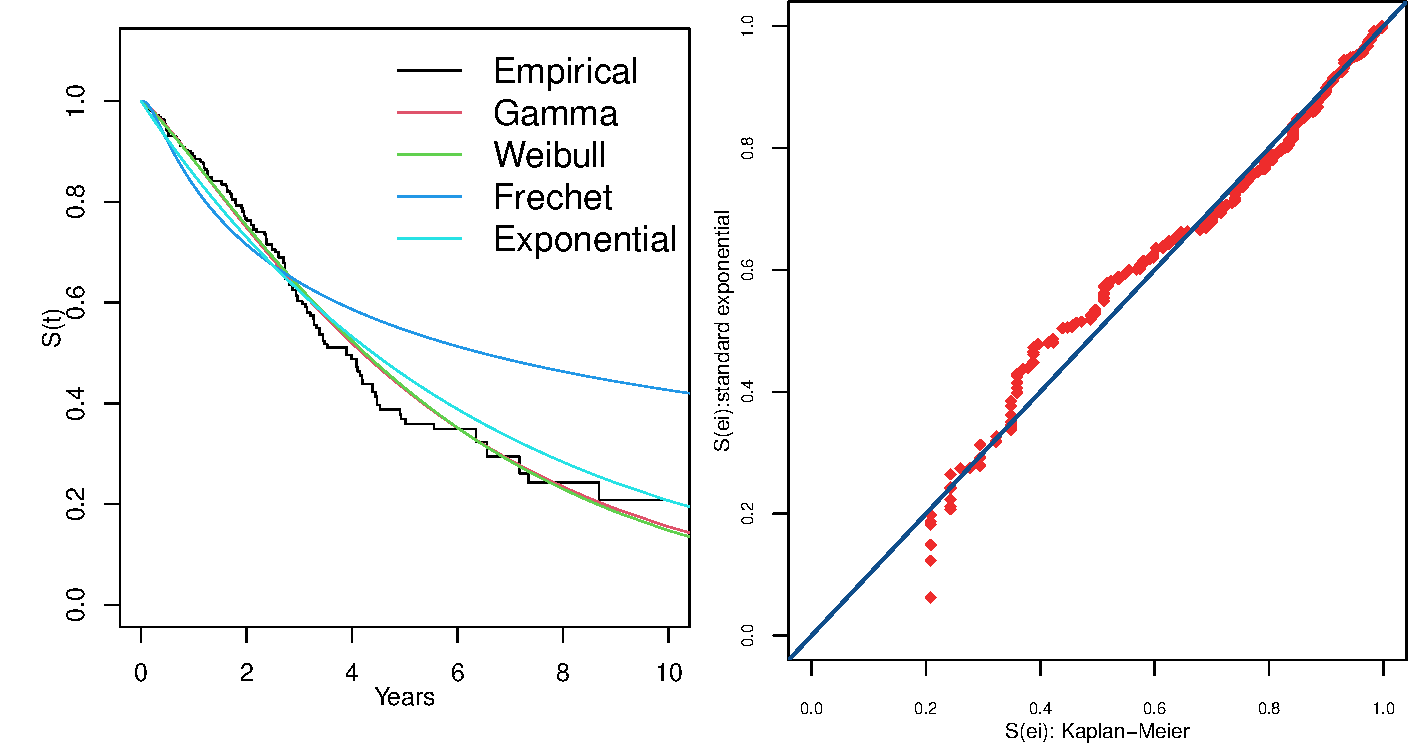
\includegraphics[scale=0.50]{survival.pdf}
	\caption{Event counts by patient lifetime. The solid
black line represents the Kaplan-Maier (KM) empirical distribution. The red line
represents the Gamma distribution, the green the Weibull, the blue line the Frechet distribution and light-green line the exponential model. The
Gamma returned closer curves to the empirical distribution, then better adjusted to the
presented data}\label{grafico-obscajust1}
\end{figure*}

Additionally, we can observe above the graphical representation of the Kaplan-Meier and standard exponential survival curves, both fitted to the Cox-Snell residuals. Notably, a significant portion of the data points lies above the reference line, indicating a strong fit of the Gamma distribution to the examined dataset. Therefore, our proposed methodology can be successfully applied to analyze the lifespan (measured in years) of patients older than 70 years diagnosed with lung adenocarcinoma, using the Gamma distribution with the objective Bayesian approach.

\section{Conclusions}\label{sec:6}

This study explores the properties of the posterior distribution of the Gamma distribution in the presence of both complete and censored data. We propose necessary and sufficient conditions to determine if an improper prior distribution leads to a proper posterior distribution. Interestingly, we find that the propriety of the posterior distribution can be established by examining only the behavior of the prior distribution. Additionally, we provide sufficient conditions to ascertain whether the higher moments of the posterior distribution are finite or infinite assuming censored data.

This study focuses on the application of the main theorem to various types of objective priors, including the uniform prior and Jeffreys first rule prior. We specifically address the challenge posed by censoring, which reveals that the Jeffreys prior becomes complex in the presence of multiple censoring. To overcome this complexity, we explore priors derived assuming complete data, which possess desirable invariant properties. Our theorem can be effectively applied using the Jeffreys prior, MDIP, and reference priors. Remarkably, our analysis demonstrates that among the considered priors, only the MDIP leads to an improper posterior distribution, while the remaining priors consistently result in proper posterior distributions.

In our study, we utilize Markov Chain Monte Carlo (MCMC) methods, specifically the Metropolis-Hastings algorithm, to obtain posterior summaries. This approach allows us to effectively explore the posterior distribution of the parameters and obtain reliable estimates. To enhance the convergence of our MCMC algorithm, we propose a novel approximate closed-form estimator specifically designed for situations involving censoring. This estimator provides excellent initial values for the iterative process, thereby improving the efficiency of the MCMC algorithm. Importantly, when there is no censoring, the estimator reduces to the ordinary closed-form maximum likelihood estimator, demonstrating its versatility and applicability in various scenarios.

To evaluate the effectiveness of our Bayesian estimators, we conduct a simulation study that compares their efficiency under different priors. This analysis enables us to assess the performance of the Bayesian approach in estimating the model parameters and to gauge the impact of prior specifications on the results.


We have applied our proposed approach to a dataset related to lung adenocarcinoma, a subtype of non-small cell lung cancer, extracted from the Cancer Genome Atlas (TCGA). Our analysis specifically targeted patients older than 70 years, aiming to explore the association between lung adenocarcinoma and lifespan. This examination provided valuable insights into disease progression and mortality frequency patterns in this specific population. Furthermore, it allowed us to identify significant patterns, relevant trends, and potential prognostic markers, which can be utilized for risk stratification and personalized medical care. This application of our methodology not only demonstrates its effectiveness and applicability in a practical context but also contributes to a deeper understanding of lung adenocarcinoma in the elderly population.


\section*{Appendix}

The following proposition gives us a relation between Definition \ref{definition0} and Definition \ref{definition1}.

\begin{proposition}\label{proportional2} Let $\f{g}:(a,b)\to\mathbb{R^+_*}$ and $\f{h}:(a,b)\to\mathbb{R^+_*}$ be continuous functions in $(a,b)\subset\mathbb{R}$, where $a\in\overline{\mathbb{R}}$ and $b\in\overline{\mathbb{R}}$, and let $c\in(a,b)$. Then, if either $\f{g}(x)\underset{x\to a}{\propto} \f{h}(x)$ or $\f{g}(x)\underset{x\to b}{\propto} \f{h}(x)$, it will follow respectively that
\begin{equation*}
\int_a^c g(x)\; dx \propto \int_a^c h(x)\; dx\ \mbox{ or }\ \int_c^b g(x)\; dx \propto \int_c^b h(x)\; dx \,.
\end{equation*}
\end{proposition} 

Using these propositions we can prove Theorem \ref{mainth} as follows:

\begin{proof} Due to the Fubini-Tonelli Theorem (see \cite{folland}) we have:

\begin{align*}%\label{posteriord2}
d(\boldsymbol{t,\delta})=&\int_{0}^{\infty}\int_{0}^{\infty}\pi(\phi,\mu)\frac{\mu^{m\phi}}{\Gamma(\phi)^n}\left\{\prod_{i=1}^n{t_i^{\delta_i(\phi-1)}}\right\}\exp\left\{-\mu\sum_{i=1}^n {\delta_i}t_i\right\}\nonumber \\
&\times \prod_{i=1}^n\left(\Gamma(\phi,\mu t_i)\right)^{1-\delta_i}d\phi d\mu.
\end{align*}
From this we can prove each item of the theorem, as follows:

\vspace{0.3cm}
\noindent \textbf{Item (i):} Suppose without loss of generality that $t_1,\cdots,t_n$ are ordered so that $\delta_i=0$ for $1\leq i\leq m-n$ and $\delta_i=1$ otherwise. Now, from the change of variables $t=\mu s$ over integration it follows from the definition of the upper incomplete gamma function that
\begin{equation*}\Gamma[\phi,\mu z] =\int_{\mu z}^\infty t^{\phi-1} e^{-t}  dt =  \int_z^\infty \mu^\phi s^{\phi-1} e^{-zs} ds
\end{equation*}
Thus, letting $\mathcal{I}=[t_1,\infty]\times \cdots \times [t_{n-m},\infty]$ and $\boldsymbol{s} = (s_1,\cdots,s_{n-m})$, since all functions under the integrand are non-negative, it follows from the Fubini-Tonelli Theorem it follows that
\begin{equation*} \prod_{i=1}^n\left(\Gamma(\phi,\mu t_i)\right)^{1-\delta_i} = \int_{\mathcal{I}} \mu^{m-n} \left\{\prod_{i=1}^{m-n} s_i \right\}^{\phi-1}e^{-\mu \sum_{i=1}^{m-n} s_i}d\boldsymbol{s}.
\end{equation*}
Thus, denoting $s_i = t_i$ for $i>n-m$, since $-1-k>0$ by hypothesis, it follows that 
 \begin{equation}
 \begin{aligned}
 \label{posteriord2}
d(\boldsymbol{t,\delta})\propto \int_{\mathcal{I}} \int_{0}^{\infty}\int_{0}^{\infty}\pi(\phi)\frac{\mu^{n\phi+k}}{\Gamma(\phi)^n}\left\{\prod_{i=1}^n{s_i}\right\}^{\phi-1}\exp\left\{-\mu\sum_{i=1}^n s_i\right\}d\phi d\mu d\boldsymbol{s} \\
\geq \int_{\mathcal{I}} \int_{0}^{\frac{-1-k}{n}}\frac{\pi(\phi)}{\Gamma(\phi)^n}\left\{\prod_{i=1}^n{s_i}\right\}^{\phi-1}\int_{0}^{1}\mu^{n\phi+k}\exp\left\{-\mu\sum_{i=1}^n s_i\right\}d\mu d\phi d\boldsymbol{s}
\end{aligned}
\end{equation}
But, since $e^{-s\mu} \underset{\mu \to 0^+}{\propto} 1$ for any $s\in\R$ it follows from Proposition \ref{proportional2} that for all $0<\phi<\frac{-1-k}{n}$ and $\boldsymbol{s}\in \mathcal{I}$ we have:
\begin{equation*}
 \begin{aligned}
\int_0^1 \mu^{n\phi+k}\exp\left\{-\mu\sum_{i=1}^n s_i\right\} d\mu
\propto \int_0^1 \mu^{n\phi+k} d\mu = \infty
\end{aligned}
\end{equation*}
since here $n\phi+k<-1$ due to the fact that we choose $\phi<\frac{-1-k}{n}$. Combining this with (\ref{posteriord2}) we conclude the posterior to be improper, which concludes item $(i)$.

\vspace{0.3cm}
\noindent \textbf{Item (ii)} By using the same development from item $(i)$ we reach
 \begin{equation}
 \begin{aligned}
 \label{posteriord3}
d(\boldsymbol{t,\delta})\propto \int_{\mathcal{I}} \int_{0}^{\infty}\int_{0}^{\infty}\pi(\phi)\frac{\mu^{n\phi+k}}{\Gamma(\phi)^n}\left\{\prod_{i=1}^n{s_i}\right\}^{\phi-1}\exp\left\{-\mu\sum_{i=1}^n s_i\right\}d\phi d\mu d\boldsymbol{s} \\
\geq \int_{\mathcal{I}} \int_{0}^{\infty}\exp\left\{-\mu\sum_{i=1}^n s_i\right\}     \int_{0}^{1}\frac{\pi(\phi)}{\Gamma(\phi)^n}\mu^{n\phi+k}\left\{\prod_{i=1}^n{s_i}\right\}^{\phi-1} d\phi  d\boldsymbol{s}
\end{aligned}
\end{equation}
Now note that for fixed $\mu>0$ and fixed $\boldsymbol{s}$ we have $\mu^{n\phi+k}\underset{\phi\to 0^+}{\propto} 1$ and $\left\{\prod_{i=1}^n{s_i}\right\}^{\phi-1}\underset{\phi\to 0^+}{\propto} 1$. Moreover, since $\Gamma(\phi)\underset{\phi \to 0}{\propto} \frac{1}{\phi}$ (see Abramowitz and Stegun \cite{abramowitz}) it follows from Propositions \ref{properties} and \ref{proportional2} that
\begin{equation*}
\int_{0}^{1}\frac{\pi(\phi)}{\Gamma(\phi)^n}\mu^{n\phi+k}\left\{\prod_{i=1}^n{s_i}\right\}^{\phi-1} d\phi  \propto \int_{0}^{1}\pi(\phi)\phi^n\; d\phi.
\end{equation*}
Finally, using the change of variables $u=\phi^{-1}\Leftrightarrow du=-\phi^{-2}\; d\phi$ it follows that
\begin{equation*} \int_{0}^{1}\pi(\phi)\phi^n\; d\phi = \int_1^\infty \pi(u^{-1})u^{-n-2}\; du = \infty
\end{equation*}
since $\lim_{u\to \infty} \pi(u^{-1})u^{-n-2} = \lim_{\phi\to 0^+} \pi(\phi)\phi^{n+2} = \infty$ by hypothesis. Combining this with (\ref{posteriord3}), we conclude the posterior to be improper, which concludes item $(ii)$.

\vspace{0.3cm}
\noindent \textbf{Item (iii)} Suppose without loss of generality that $t_1,\cdots,t_n$ are ordered so that $\delta_i=1$ for $1\leq i\leq m$ and $\delta_i=0$ otherwise. Since $\Gamma[\phi,z]\leq \Gamma(\phi)$ for all $z\geq 0$ it follows that

%\begin{equation}
%\begin{aligned}
%\label{posteriord2}
%d(\boldsymbol{t,\delta})=\int_{0}^{\infty}\int_{0}^{\infty}\pi(\phi,\mu)\frac{\mu^{m\phi}}{\Gamma(\phi)^n}\left\{\prod_{i=1}^m{t_i^{\phi-1}}\right\}\exp\left\{-\mu\sum_{i=1}^m t_i\right\}\prod_{i=1}^n\left(\Gamma(\phi,\mu t_i)\right)^{1-\delta_i}d\phi d\mu \\
%\leq \int_{0}^{\infty}\int_{0}^{\infty}\pi(\phi,\mu)\frac{\mu^{m\phi}}{\Gamma(\phi)^m}\left\{\prod_{i=1}^m{t_i^{\phi-1}}\right\}\exp\left\{-\mu\sum_{i=1}^m t_i\right\}d\phi d\mu\\
%= \int_{0}^{\infty}\pi(\phi)\frac{\Gamma(m\phi)}{\Gamma(\phi)^m}\left\{\prod_{i=1}^m{t_i^{\phi-1}}\right\}\left\{\sum_{i=1}^m t_i\right\}^{-m\phi} d\phi\\
%= c \int_{0}^{\infty}\pi(\phi)\frac{\Gamma(m\phi)}{\Gamma(\phi)^m m^{m \phi}}e^{-p\phi} d\phi
%\end{aligned}
%\end{equation}

\begin{align*}
%\label{posteriord2}
d(\boldsymbol{t,\delta})\propto &\int_{0}^{\infty}\int_{0}^{\infty}\pi(\phi)\mu^k\frac{\mu^{m\phi}}{\Gamma(\phi)^n}\left\{\prod_{i=1}^m{t_i^{\phi-1}}\right\}\exp\left\{-\mu\sum_{i=1}^m t_i\right\}\prod_{i=1}^n\left(\Gamma(\phi,\mu t_i)\right)^{1-\delta_i}d\phi d\mu \nonumber\\
&\leq \int_{0}^{\infty}\int_{0}^{\infty}\pi(\phi)\frac{\mu^{m\phi+k}}{\Gamma(\phi)^m}\left\{\prod_{i=1}^m{t_i^{\phi-1}}\right\}\exp\left\{-\mu\sum_{i=1}^m t_i\right\}d\phi d\mu \nonumber\\
&= \int_{0}^{\infty}\pi(\phi)\frac{\Gamma(m\phi)}{\Gamma(\phi)^m}\left\{\prod_{i=1}^m{t_i^{\phi-1}}\right\}\left\{\sum_{i=1}^m t_i\right\}^{-m\phi} d\phi \nonumber \\
&= c \int_{0}^{\infty}\pi(\phi)\frac{\Gamma(m\phi)}{\Gamma(\phi)^m m^{m \phi}}e^{-p\phi}\; d\phi,
\end{align*}
where $c = \frac{1}{\prod_{i=1}^m t_i}$ 
and $p = m \log\left(\frac{\frac{1}{m}\sum_{i=1}^m t_i}{\sqrt[n]{\prod_{i=1}^m t_i}}\right)$ is a positive value due to the arithmetic-geometric mean inequality and the hypothesis that $m>0$ and that the uncensored times $t_1,\cdots,t_m$ are not all equal.

Now, letting $g(\phi)=\pi(\phi)\frac{\Gamma(m\phi)}{\Gamma(\phi)^m m^{m \phi}}e^{-p\phi}$ we have
\begin{equation*} \int_{0}^{\infty}\pi(\phi)\frac{\Gamma(m\phi)}{\Gamma(\phi)^m m^{m \phi}}e^{-p\phi}\; d\phi =  \int_{0}^1g(\phi)\; d\phi + \int_1^\infty g(\phi)\; d\phi = s_1+s_2.
\end{equation*}
and we shall prove that $s_1<\infty$ and $s_2<\infty$. Indeed, since
 $e^{-p\phi}m^{-m\phi}\underset{\phi\to 0^+}{\propto}1$ and $\Gamma(x)\underset{\phi\to 0^+}{\propto} \frac{1}{x}$ it follows from Propositions \ref{properties} and \ref{proportional2} that
 \begin{equation*} s_1=\int_{0}^1 g(\phi)\; d\phi \propto \int_0^1 \phi^{r_0}\frac{\frac{1}{m\phi}}{\left(\frac{1}{\phi}\right)^m}\; d\phi \propto \int_0^1 \phi^{r_0+m-1}\; d\phi < \infty
 \end{equation*}
since $r_0+m-1>-1$ by hypothesis. Finally, since from the Stirling approximation of the Gamma function, we have $\Gamma(x)\underset{\phi\to \infty}{\propto} x^{x-\frac{1}{2}}e^{-x}$ (see Abramowitz and Stegun \cite{abramowitz}) we have, once again due to Propositions \ref{properties} and \ref{proportional2} that
\begin{equation*}
\begin{aligned}
s_2 = \int_1^\infty g(\phi)\; d\phi \propto \int_{1}^{\infty}\phi^{r_\infty}\frac{(m\phi)^{m\phi-\frac{1}{2}}e^{-m\phi}}{\phi^{m\phi-\frac{m}{2}}e^{-m\phi} m^{m \phi}}e^{-p\phi}\; d\phi\\ = m^{-\frac{1}{2}} \int_1^\infty \phi^{r_\infty+\frac{m+1}{2}-1}e^{-p\phi}\; d\phi = m^{-\frac{1}{2}}\frac{\Gamma\left(r_\infty+\frac{m+1}{2},p\right)}{p^{r_\infty+\frac{m+1}{2}}}<\infty
\end{aligned}
\end{equation*}
which proves that $s_2<\infty$, concluding the proof that $d(\boldsymbol{t,\delta})<\infty$.
\end{proof}


%\begin{acknowledgements}
%If you'd like to thank anyone, place your comments here
%and remove the percent signs.
%\end{acknowledgements}

% BibTeX users please use one of
\bibliographystyle{unsrtnat}      % basic style, author-year citations
\bibliography{reference}   % name your BibTeX data base


% Non-BibTeX users pl

\end{document}
% end of file template.tex

